\subsection{One dimensional hydrogen chain}
We now move to one of the simplest extended \emph{ab-initio} systems, a hydrogen chain with periodic boundary conditions. 
In the absence of availability of exact eigenstates, the example will highlight the effectiveness of the N-AIDMD approach.
We consider the case of $10$ atoms and work in a regime where the inter-atomic distance $r$ is 
relatively large ($r=1.5$ to $3.0$ \AA), such that the system is potentially well described by a 1-band Hubbard model 
in terms of primarily $s$-like orbitals, whose form we discuss here. 

For a given $r$, we first obtain single-particle Kohn-Sham orbitals from a set of spin-unrestricted and 
spin-restricted DFT-PBE calculations. The localized orbital basis upon which the descriptors (density matrices) 
are calculated is obtained by generating intrinsic atomic orbitals (IAO) from the Kohn-Sham orbitals, and orthogonalizing them using 
the L\"owdin procedure; our results are shown in Fig.~xx \HHZ{Could you plot these orbitals and replace the Wannier orbitals stuff?}
These form the effective orbitals that enter the 1-band Hubbard Hamiltonian. 

\begin{figure}[]
\centering
\subfigure[KS 1]{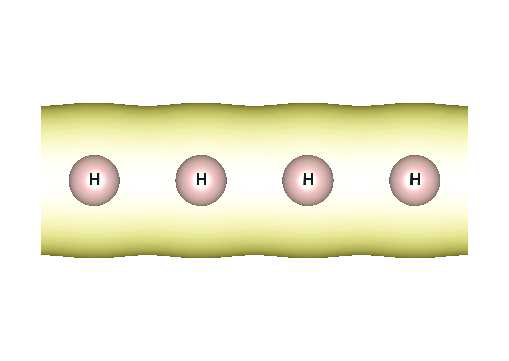
\includegraphics[width=0.20\linewidth]{./Figures/h4_ks1.png}}\quad
\subfigure[KS 2]{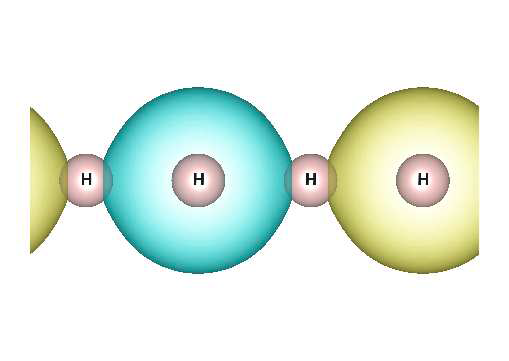
\includegraphics[width=0.20\linewidth]{./Figures/h4_ks2.png}}\quad
\subfigure[KS 3]{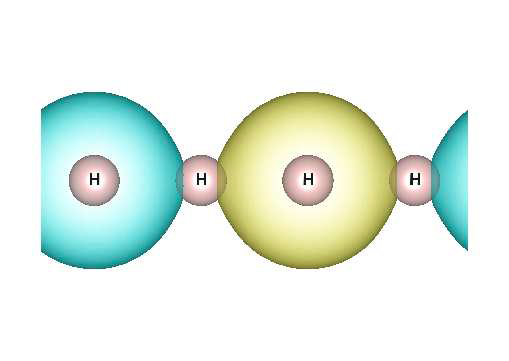
\includegraphics[width=0.20\linewidth]{./Figures/h4_ks3.png}}\quad
\subfigure[KS 4]{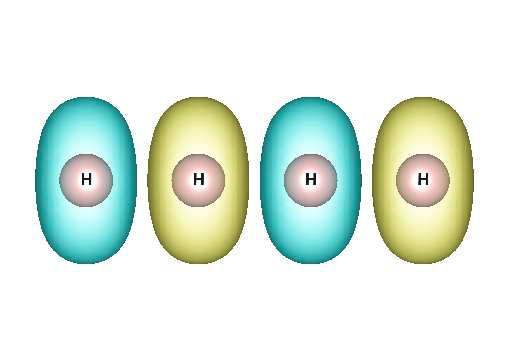
\includegraphics[width=0.20\linewidth]{./Figures/h4_ks4.png}}
\\
\subfigure[Wannier 1]{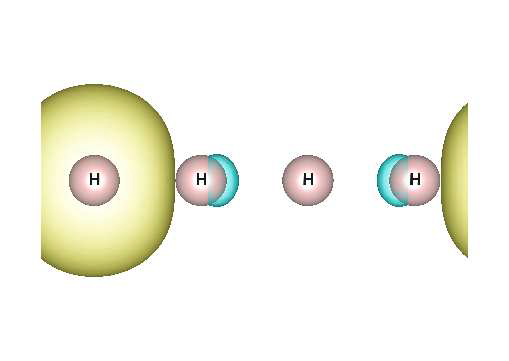
\includegraphics[width=0.20\linewidth]{./Figures/h4_wan1.png}}\quad
\subfigure[Wannier 2]{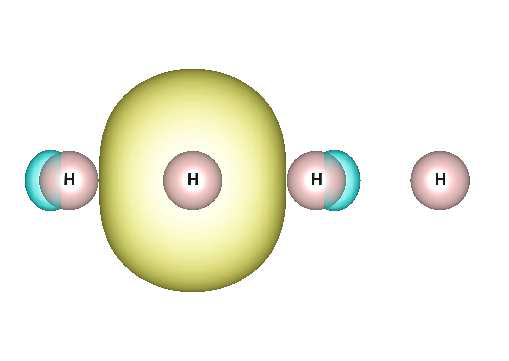
\includegraphics[width=0.20\linewidth]{./Figures/h4_wan2.png}}\quad
\subfigure[Wannier 3]{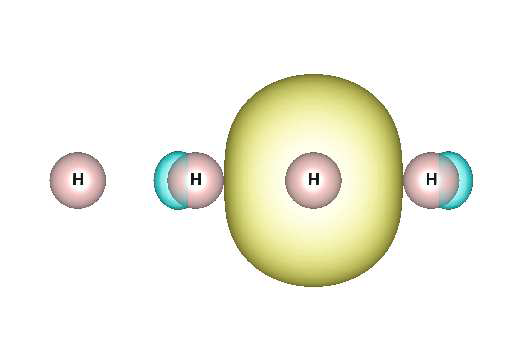
\includegraphics[width=0.20\linewidth]{./Figures/h4_wan3.png}}\quad
\subfigure[Wannier 4]{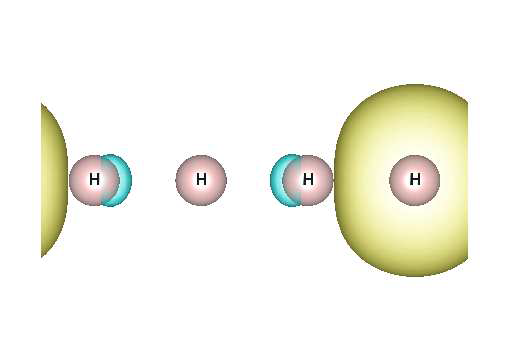
\includegraphics[width=0.20\linewidth]{./Figures/h4_wan4.png}}
\caption{\HJC{Put IAO here} Kohn-Sham orbitals (upper panel) from DFT calculations with PBE exchange-exchange correlation functional, and Wannier orbitals (lower panel) constructed through a unitary transformation of Kohn-Sham orbitals.}\label{fig:h4orb}
\end{figure}


To generate a database of wavefunctions needed for the N-AIDMD, 
we produce a set of wavefunctions (\HHZ{Slater-Jastrow wave functions?}) consisting of singles- and doubles- excitations 
to the Slater determinant, 
\begin{subequations}
\begin{eqnarray}
| s \rangle = & \Big[a^\dagger_{i \sigma} a_{k \sigma}   | KS \rangle \Big]e^J \\
| d \rangle = & \: \Big[a^\dagger_{i \sigma} a^\dagger_{j \sigma'} a_{k \sigma'} c_{l \sigma}   | KS \rangle\Big]e^J ,
\end{eqnarray}
\end{subequations}
where $|KS\rangle$ is the Stater determinant of occupied Kohn-Sham orbitals, $\sigma$ and $\sigma'$ are spin indices, 
and $a_{i}^\dagger$ ($a_{i}$) is a single-electron creation (destruction) corresponding to Kohn-Sham orbitals, 
and $e^J$ is the Jastrow factor which was optimized using variational Monte Carlo. 
Then, having computed the energies (expectation values of the Hamiltonian) and corresponding 
descriptors for these wavefunctions we verify the independence of the $U$ and $t$ descriptors.
We then fit the 1-band Hubbard Hamiltonian using least-squares fitting, as part of the formalism described in sec. 2. 

\begin{figure}
\centering
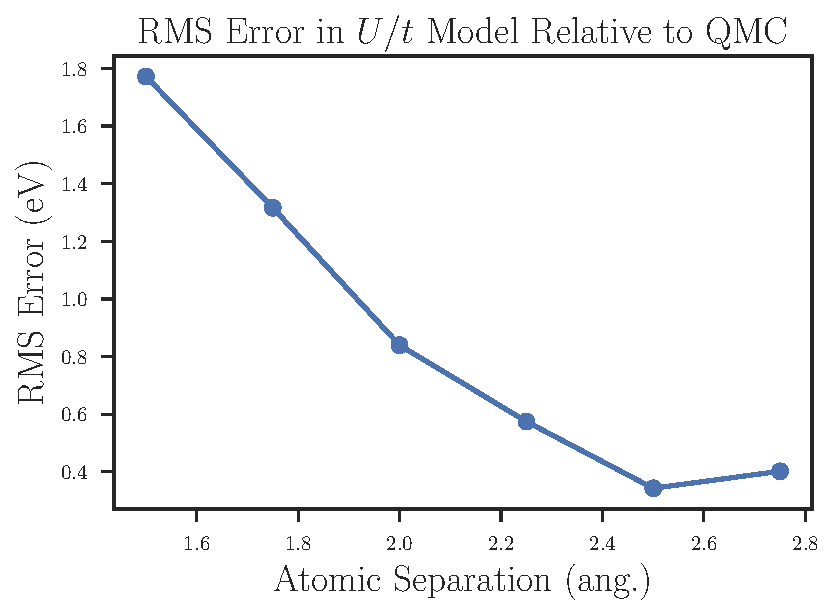
\includegraphics[scale=0.5]{./Figures/rms_ut_error_vs_separation_h_chain.pdf}
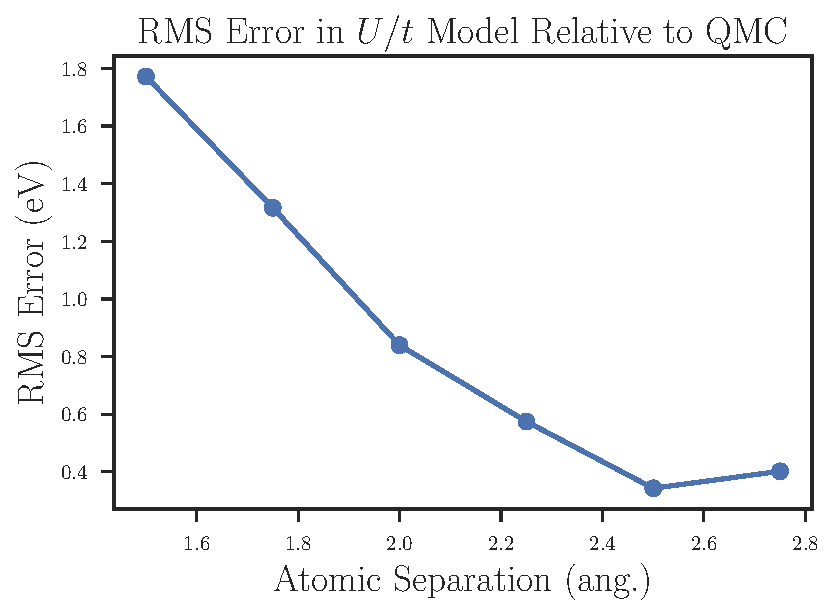
\includegraphics[scale=0.5]{./Figures/rms_ut_error_vs_separation_h_chain.pdf}
\caption{\HJC{Put model vs ab-initio plots here}The RMS error in the fitted $U$-$t$ model for the periodic H$_{10}$ chain, relative to the \textit{ab-initio} energies. The RMS error is less than 1 eV for sufficiently long bond lengths.}\label{fig:fit_quality}
\end{figure}
Fig.~\ref{fig:fit_quality} shows our N-AIDMD fits for two representative $r$. As expected, the RMS error 
is significantly smaller for larger $r$, verifying the effectiveness of the Hubbard model 
in this limit. 

Fig.~\ref{fig:Parameters-vs-Bond-t} also shows trends of the fitted value of the one-body hopping $t$ 
and the repulsion $U$ as a function of $r$. Consistent with physical intuition, $t$ decreases towards zero at larger $r$
and the value of $U/t$ rises. Based on these values and the extensive body of work in 1D systems we expect a Luttinger liquid 
to insulator transition to occur at $U/t=...$ corresponding to $r=...$.  

\begin{figure}
\centering
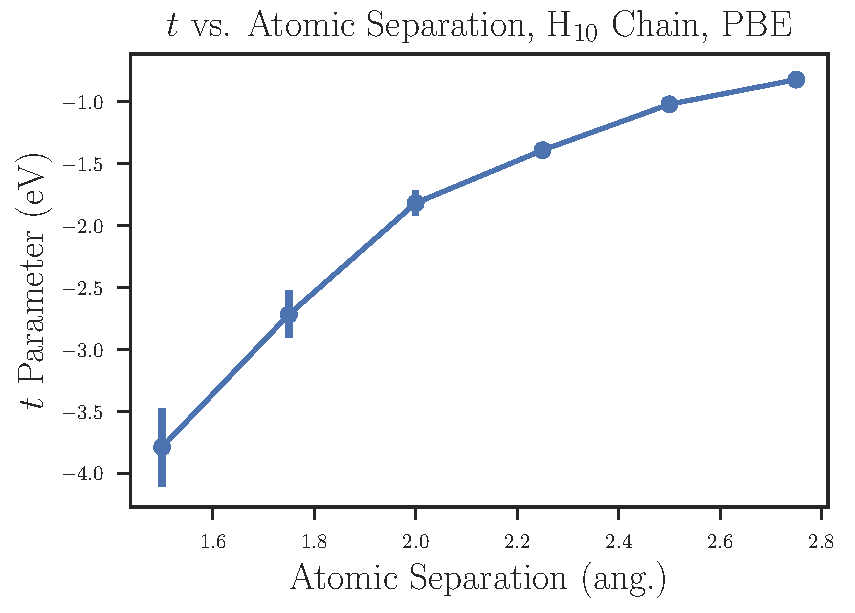
\includegraphics[scale=0.5]{./Figures/$t$_vs_separation_h_chain_ols.pdf}
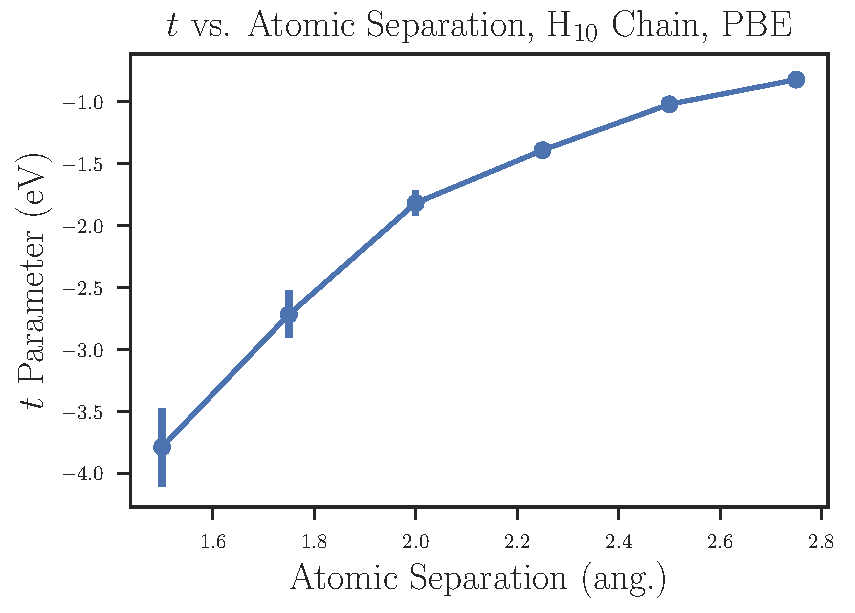
\includegraphics[scale=0.5]{./Figures/$t$_vs_separation_h_chain_ols.pdf}
\caption{\HJC{Put t vs r and U/t vs r} The one-body hopping $t$ parameter as a function of lattice constant for the periodic H$_{10}$ chain, obtained from a fitted $U$-$t$ model. The parameter value declines to zero as the lattice constant increases. \HHZ{I suggest to remove the titles from the figure, and put description in the caption instead. The y-axis label: how about "Hopping parameter $t$"}}\label{fig:Parameters-vs-Bond-t}

\end{figure}
